\documentclass[10pt,addpoints]{exam} %% no solution

\usepackage{mathtools}
\usepackage{amsmath}
\usepackage{amssymb}
\usepackage{xcolor}
\usepackage{graphicx}
\usepackage[top=2.0cm,bottom=2.0cm,left=2.5cm,right=2.5cm]{geometry}
\usepackage{tikz}
\usepackage{float}
\usepackage{multicol}
\usepackage{pgfplots}
\usepackage{lastpage}
\usepackage{soul}
\usepackage{libertine}
\usepackage{lipsum}
\usepackage{siunitx}
\usepackage{xspace}
\newenvironment{Figure}
  {\par\medskip\noindent\minipage{\linewidth}}
  {\endminipage\par\medskip}
\usepackage[labelfont=bf]{caption}
\usepackage[hidelinks, urlcolor=blue, linkcolor=black, colorlinks=true]{hyperref}
\usepackage[capitalize,noabbrev]{cleveref}
\usepackage[absolute]{textpos}

\usepackage[normalem]{ulem}

\newcommand{\todo}[1]{\hl{\textbf{ToDo:}~#1}}

%% define course title
\newcommand{\course}{MAT185}
\newcommand{\assignmenttitle}{Assignment 2}

%% header and footer
\firstpageheader{}{}{\textbf{{\color{red} Due}: 10:00pm, Tuesday Feb. 4, 2025}}
\firstpageheadrule
\runningheader{}{Page~\thepage~of~\numpages}{\course~--~\assignmenttitle}
\footer{}{}{}

\setlength\parindent{0pt} % no indentation in document

%% formats exam class
\qformat{\textbf{Question \thequestiontitle:}\hfill} % title of question 
\boxedpoints
\pointpoints{mark}{marks}
\pointsinrightmargin
\hpword{Marks:}
\hsword{Your score:}
\unframedsolutions
\totalformat{\boxed{\textnormal{\totalpoints~\if\totalpoints1 mark\else marks\fi}}}
\definecolor{SolutionColor}{rgb}{0,0,1}
\renewcommand{\solutiontitle}{}
\AtBeginEnvironment{solution}{\color{blue}}

% %correct choices in solution
\CorrectChoiceEmphasis{\rm}
\checkedchar{\tikz\draw[blue,fill=blue] (0,0) circle (1ex);}

% %
\newcommand{\mblue}[1]{\color{blue}\textit{#1}\color{black}}

% % increase distance between checkbox items
\renewcommand{\checkboxeshook}{\setlength{\itemsep}{6pt}}

%% distance between questions and parts
\renewcommand{\questionshook}{\setlength{\parsep}{10pt}}
\renewcommand{\partshook}{\setlength{\parsep}{15pt}}

%% define arrows in text
\newcommand{\arrow}{$\rightarrow$\xspace}
\newcommand{\Arrow}{$\Rightarrow$\xspace}

% % math notation:
%\veccol{1}{2}{3}
\newcommand{\veccol}[3]{
    \begin{bmatrix}
        #1\\
        #2\\
        #3\\
    \end{bmatrix}}
  
%\vecrow{1}{2}{3}
\newcommand{\vecrow}[3]{\left[#1~#2~#3\right]}

%\matrixTwo{1}{2}{3}{4}
\newcommand{\matrixTwo}[4]{\left[\begin{array}{cc}#1&#2\\#3&#4\end{array}\right]}

% \matrixThree{1}{2}{3}{4}{5}{6}{7}{8}{9}
\newcommand{\matrixThree}[9]{\left[\begin{array}{ccc}#1&#2&#3\\#4&#5&#6\\#7&#8&#9\end{array}\right]}

%\matrixCorner{1}{2}{3}{4}
\newcommand{\matrixCorner}[4]{\left[\begin{array}{ccc}#1& \cdots&#2\\ \vdots & \ddots & \vdots\\#3&
      \cdots&#4\end{array}\right]}
      
% real numbers
\newcommand{\R}{\mathbb{R}}

% \nR
\newcommand{\nR}{{}^{n}\mathbb{R}}
% \mR
\newcommand{\mR}{{}^{m}\mathbb{R}}
% \Rn
\newcommand{\Rn}{\mathbb{R}^{n}}
% \nRn
\newcommand{\nRn}{{}^{n}\mathbb{R}^{n}}
% \nRm
\newcommand{\nRm}{{}^{n}\mathbb{R}^{m}}
% \nRm
\newcommand{\mRn}{{}^{m}\mathbb{R}^{n}}
% \mRm
\newcommand{\mRm}{{}^{m}\mathbb{R}^{m}}                              
       
%% define abbreviations
\newcommand{\row}{\operatorname{row}\,}
\newcommand{\col}{\operatorname{col}\,}
\renewcommand{\dim}{\operatorname{dim}\,}
\renewcommand{\span}{\operatorname{span}\,}
\newcommand{\rank}{\operatorname{rank}\,}
\renewcommand{\ker}{\operatorname{ker}\,}
\newcommand{\nul}{\operatorname{null}\,}
\renewcommand{\det}{\operatorname{det}\,}
\newcommand{\adj}{\operatorname{adj}\,}

%%% This command makes a framed box of a chosen height.
\newcommand{\makenonemptybox}[2]{%
\par\nobreak\vspace{\ht\strutbox}\noindent
\setlength{\fboxrule}{0pt} % set this to 0pt to make invisible
\fbox{%
\parbox[c][#1][t]{\dimexpr\linewidth-2\fboxsep}{
  \hrule width \hsize height 0pt
  \vspace{-0.6cm}
  \color{SolutionColor}#2\color{black}
 }%
}%
}

  
\begin{document}

\vspace*{-0.5cm}
\begin{center}
  \large
  \textbf{\Large \course~--~Linear Algebra}\\[0.1cm]
  \textbf{\assignmenttitle}
\end{center}
\bigskip

\textbf{\large Instructions:}\\
\normalsize

Please read the {\bf MAT185 Assignment Policies \& FAQ} document for
details on submission policies, collaboration rules and academic integrity, and
general instructions.

\begin{enumerate}


\item \textbf{Submissions are only accepted by}
  \href{https://www.gradescope.ca}{Gradescope}. Do not send anything by email.
  Late submissions are not accepted under any circumstance. Remember you can
  resubmit anytime before the deadline.

\item \textbf{Submit solutions using only this template pdf}.  Your submission
  should be a single pdf with your full written solutions for each question. If
  your solution is not written using this template pdf (scanned print or
  digital) then your submission will not be assessed. Organize your work neatly
  in the space provided.  Do not submit rough work.

\item \textbf{Show your work and justify your steps} on every question but do
  not include extraneous information.  Put your final answer in the box
  provided, if necessary.  We recommend you write draft solutions on separate
  pages and afterwards write your polished solutions here on this template.

\item \textbf{You must fill out and sign the academic integrity statement
    below}; otherwise, you will receive zero for this assignment.

\end{enumerate}

\vspace{10pt}


\textbf{\large Academic Integrity Statement:} \\

%%% Student information

% Student 1
\fbox{
  \begin{minipage}{\textwidth}
    \vspace{0.75cm}
    \makebox[\textwidth]{\large Full Name: CHEUNG, Hei Shing (Hayson)\enspace\hrulefill}\\[0.75cm]
    \makebox[\textwidth]{\large Student number: 1010907823\enspace\hrulefill}\\
  \end{minipage}
}

\vspace*{0.1in}

% Student 2
\fbox{
  \begin{minipage}{\textwidth}
    \vspace{0.75cm}
    \makebox[\textwidth]{\large Full Name: SIU, Nelson\enspace\hrulefill}\\[0.75cm]
    \makebox[\textwidth]{\large Student number: 1010940608 \enspace\hrulefill}\\
  \end{minipage}
}

\bigskip
\large \textbf{I confirm that:}
\normalsize

\begin{itemize} 
\item I have read and followed the policies described in the document {\bf
    MAT185 Assignment Policies \& FAQ}.
\item In particular, I have read and understand the rules for
  collaboration, and permitted resources on assignments as described in
  subsection II of the the aforementioned document. I have not violated
  these rules while completing and writing this assignment.
\item I have not used generative AI in writing this assignment.
\item I understand the consequences of violating the University's academic
  integrity policies as outlined in the
  \href{http://www.governingcouncil.utoronto.ca/policies/behaveac.htm}{Code of
    Behaviour on Academic Matters}. I have not violated them while completing
  and writing this assignment.
\end{itemize}
\bigskip

\large \textbf{By submitting this assignment to Gradescope, I agree that the
  statements above are true.}  \normalsize

\newpage

\section*{Preamble:}

Image processing is the manipulation of digital images by applying mathematical tools and
algorithms. A wide range of applications based on digital image processing are, for example, medical
imaging, image optimization in consumer cameras, computer vision, and satellite imagery. Linear
algebra, and the techniques you will learn during this course, plays a crucial role in that field by
providing a mathematical foundation.\\

A typical digital image can be considered as a 2-dimensional matrix of \textit{pixels} (abbreviation
for \textit{picture element}). Methods of digital image processing are manipulating this
2D-matrix. A pixel is the smallest element of a digitally acquired raster image, and can be
considered as a colour sample at each point of an image. Typically, each pixel is represented by 3
positive integer values from 0 to 255 for each colour red, green, and blue: 0 is representing black
and 255 ($= 2^8-1$) either red, green, or blue. In that case, 24 Bits are used to code 16,777,216
distinct colours for each pixel. This is called a 24\,bpp (24\,Bits-per-pixel) colour depth. If a
grey-scale image is sampled, each pixel samples the light intensity. In that case, only 8\,Bits
(single integers from 0 to 255) are typically necessary, as shown in \cref{fig:imagematrix}, to
store grey-scale images.

\begin{figure}[H]
  \centering
  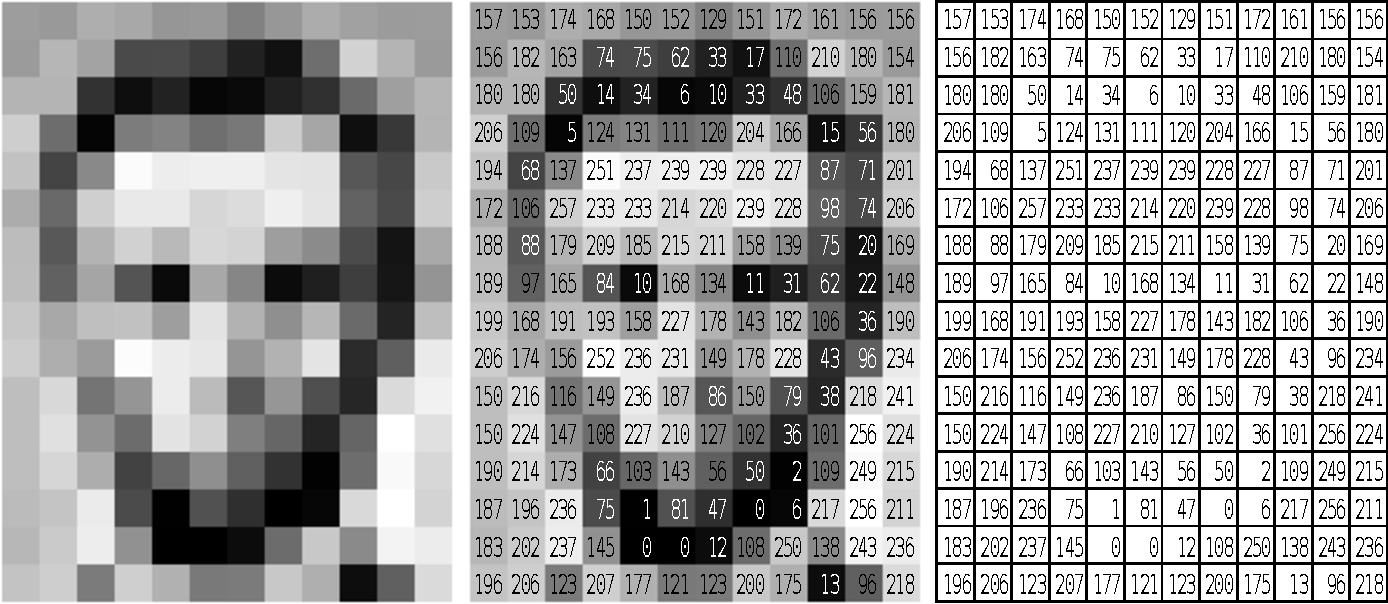
\includegraphics[width=0.9\textwidth]{imagematrix.pdf}
  \caption{Grey-scale image represented by 8 bpp
    (Bits-per-pixel). [\textit{source: stanford.edu}]}
  \label{fig:imagematrix}
\end{figure}

One application of linear algebra in the context of digital image processing is for a linear
transformation of the images / 2D-matrices. We will discuss linear transformations in more detail
later this term. Common transformations include scaling, rotation, and translation of the image. All
of these linear transformations can be represented by a matrix
multiplication.\\

Another important application of linear algebra in the context of digital image processing is
filtering, which will be explored in Question~\ref{q:filtering} of this assignment. Filtering
includes, for example, methods for noise reduction, blurring/sharpening, edge
detection, white balancing, colour correction, and many more.\\

Lastly, images have to be stored in efficient ways. For a colour image of size $n\times m$ with a
24\,bpp colour depth, $m \times n \times 24$\,Bits of memory are necessary. An image of
$8000\times 6000$ Pixels (4:3 aspect ratio and 48MP resolution of modern smartphone cameras) with
24\,Bit colour depth will lead to an uncompressed image filesize of 144\,MB. To reduce the image
filesize, lossy (permanently removing \textit{unnecessary} information of the original image) and
lossless compression methods are applied. For lossy compression algorithms, it is vital to identify
unnecessary information of the image, which are not perceived by the viewer and can be removed. One
approach for a lossy compression is based on the Singular Value Decomposition (SVD), which will be
explored in more detail in Question~\ref{q:sdv}.

\newpage

\begin{questions}
  \question\label{q:filtering} For simplicity, we assume that each
    pixel of a grey-scale image is considered as a real value in
    Question~\ref{q:filtering}(\ref{part:first}) to (\ref{part:second_last}).
  Let $G \in \nRm$ be a grey-scale image of $n \times m$ pixels. A collection of
  image filters $ F_1, F_2, \dots, F_k \in \nRm$ can be used to process this
  image, resulting in filtered images $A_l$ represented as:
  \begin{equation}
    \label{eq:filter}
    A_l = F_l \circ G, \quad l = 1, 2, \dots, k,
  \end{equation}
  where $ \circ $ denotes the entry-wise product. The entry-wise product (also called
  \textit{Hadamard} product) of two matrices of the same size is defined as the product, where each
  entry of the resulting matrix is the product of the corresponding entries of the original
  matrices.
  For example, if $P = \matrixTwo{p_{11}}{p_{12}}{p_{21}}{p_{22}}$ and
  $Q= \matrixTwo{q_{11}}{q_{12}}{q_{21}}{q_{22}}$ are $2\times 2$ matrices, the Hadamard product is
  defined as
  \begin{equation}
  P\circ Q = \matrixTwo{p_{11}q_{11}}{p_{12}q_{12}}{p_{21}q_{21}}{p_{22}q_{22}}.
\end{equation}
        
  \begin{parts}

    \part\label{part:first} Can the filter $F_1$ in \cref{eq:filter} be used to blur or smooth an image
      $A_1$? Unsupported answers will not receive full credit.
      
      %%% Do not change the height of this box. Your work must fit inside it.
      \makenonemptybox{3cm}{
        %%% Your work goes here!
        %        
        % \textbf{YES}, since $F_1$ can be anything, assume that we can compute the filter $F_1$ based on the image $A_1$.
        % We can apply a bluring algorithm to the image $G = \{g_{ij}\}$ to get the filter $F_1 = \{f_{ij}\}$. One naive way to do this is to average the pixel values in a $3\times 3$ window around each pixel:
        \textbf{YES}. Define \textit{blurring} as an operation so that the average gradient between pixels decreases. 
        Apply a blurring algorithm to the image $G = \{g_{ij}\}$ to get the filter $F_1 = \{f_{ij}\}$. 
        One naive way to do this is by averaging the each pixel values in a $3\times 3$ window, and devide by the pixel value to get the filter $F^\prime_1$, hence $F^\prime_1 \circ G$ is \textit{blurred}. 
        You specified for the same filter $F_1$ to blur the filterd image $A_1 = F_1 \circ G$ when applied as a Hadamard Product. 
        We can modify the same said averaging filter to blur both $A_1$ and $G$. We can do it by taking the root of the filter values, which allows us to gradually reuse the same filter as Haddamard product: $A_2 = F_1 \circ A_1 = F_1 \circ F_1 \circ G$. Further explanation and results: \href{https://github.com/HaysonC/svdAssignment}{https://github.com/HaysonC/svdAssignment}
        \begin{equation*}
           f_{ij} = \sqrt[3]{\frac{1}{9g_{ij}} \sum_{0\le s,t\le 2} g_{i+s-1,j+t-1}}  = \sqrt[3]{\frac{\operatorname{conv}(\{1/9\}_{3\times 3}, G)_{ij}}{g_{ij}}}
        \end{equation*}
        % Then, we can apply the filter $F_1$ to the image $G$ to get the blurred image $A_1= F_1 \circ G$ \\
        % \tiny{\\ \textbf{Note for 1(a)} Assume we can compute $F_1$ based on the entire image. Otherwise, the answer to 1(a) is \textbf{NO}, because smoothing and bluring must consider nearby pixels, element-wise multiplication cannot achieve that since each operation is independent of other pixels in the matrix. For instance, the example as shown in my solution is that of a convolutional multiplication with a $3\times3$ kernel $K = \frac{1}{9}\{1\}_{3\times3}$, which is a simple blurring kernel, with $A_1 = K \ast G$. Also, if you consider a zero matrix (black iamge) as a blured one, then for all image we can apply the the zero matrix filter.}  The filter $F_1$ would be a $3\times 3$ matrix with entries $\frac{1}{9}$.
        }
    \part Name at least \textbf{three} applications in the context of digital
    image processing for a filter as defined in \cref{eq:filter}. Additionally,
    give details how $F_i$ would look like for your applications. 

    %%% Do not change the height of this box. Your work must fit inside it.
    \makenonemptybox{10cm}{
      \begin{enumerate}
        \item \textbf{Adusting white balance/color temperature} The filter $F_i$ can be used to adjust the white balance of an image. By setting a filter to enhance the red or blue channel, we can adjust the color temperature of the image by mulitplying the filter to the specific channel. We assume that a colored image is defined as $\{R, G, B\}$, then $\{F_i\circ R, G,B\}$ will be the new image with adjusted white balance. In this case $F_i$ would be a uniform matrix with entries greater than one if we want to enhance the color, and less than one if we want to decrease the color.
        \item \textbf{Cinematic Effects} Certain filters can be used to create cinematic effects. For example, a filter that dims the edges of image (vignette) can be applied by multiplying the filter to the image. The filter will have a ones in the center and approaches zero as it goes to the edges.
        \item \textbf{Artifcially Increasing Exposure} A filter can be used to artificially increase the exposure of an image. By multiplying the filter to the image, the pixel values will be increased by a certain factor. The filter will have values greater than one, otherwise, we can use the filter to decrease the exposure. The increased exposure image will be $\{F_i\circ G\}$, and it would look like a brighter version of the original image.
      \end{enumerate}      
      
      %%% end of your answer    
    }

     
\newpage
    
\part \label{part:linind} Assume that the entries of the image $G$ are all nonzero.  Prove that the
  set of filtered images $\{F_1\circ G, F_2\circ G, \dots, F_k\circ G\}$ is linearly independent if
  and only if the set of filters $\{F_1, F_2, \dots, F_k\}$ is linearly independent.

  %%% Do not change the height of this box. Your work must fit inside it.
    \makenonemptybox{17cm}{
      %%% Your work goes here!      
      (``$\Rightarrow$") Assume, for the sake of contrapositive, that the set of filters $\{F_1, F_2, \dots, F_k\}$ is linearly dependent. Then, we proof that exists a non-trivial linear combination of the filtered images that equals the zero vector. We first consider the linear combination of the filtered images, by the Distributive Property, as:
      $$ \lambda_1(F_1\circ G) + \lambda_2(F_2\circ G) + \dots + \lambda_k(F_k\circ G)$$
      Since multiplicati on in the Hadamard product is commutative, we can consider $\lambda_j(F_j\circ G) = G\circ(\lambda_j F_j)$. We can then rewrite the linear combination as:
      $$ G\circ(\lambda_1F_1 + \lambda_2F_2 + \dots + \lambda_kF_k)$$
      Since there exist a non-trivial linear combination of the filters that equals the zero vector, we take ${\mu_1, \mu_2, \dots, \mu_k} \neq \textbf{0}_k$ such that $\mu_1F_1 + \mu_2F_2 + \dots + \mu_kF_k = 0$. We coule then pick $\lambda_j = \mu_j$ and rewrite the linear combination as:
      $$ G\circ(\mu_1F_1 + \mu_2F_2 + \dots + \mu_kF_k) = G\circ\textbf{0}$$
      Thus, since $G \neq \textbf{0}$, there also exist a non-trivial linear combination of the filtered images that equals the zero vector, which implies that the set of filtered images is linearly dependent.\\ \\
      (``$\Leftarrow$") Assume, for the sake of contrapositive, that the set of filtered images is linearly dependent. Then, we proof that there exist a non-trivial linear combination of the filters that equals the zero vector. We first consider the linear combination of the filters:
      $$ \mu_1F_1 + \mu_2F_2 + \dots + \mu_kF_k$$
      Since the images are of any real matrix of a specific size, we can take the Hadamard product of the linear combination with the image $G$, again, by the Distributive Property, we have:
      $$ G\circ(\mu_1F_1 + \mu_2F_2 + \dots + \mu_kF_k) = G\circ\textbf{0} = \textbf{0}$$
      Again, by communativity of the Hadamard product, we can rewrite the linear combination as:
      $$ \mu_1(F_1\circ G) + \mu_2(F_2\circ G) + \dots + \mu_k(F_k\circ G) = \textbf{0}$$
      Since $\{\mu_1, \mu_2, \dots, \mu_k\} \neq \textbf{0}_k$, there exist a non-trivial linear combination of the filtered images that equals the zero vector, which implies that the set of filters is linearly dependent.\\
    }

   \newpage
    
  \part Assume that the entries of the image $G$ are all nonzero.  Let $\mathcal{W}$ be the set of
    the filtered images $\{F_1 \circ G, F_2 \circ G, \dots, F_k \circ G\}$. Suppose a new image
    filter $ F_{k+1} $ is introduced. Prove that the filtered image $ F_{k+1} \circ G $ lies in
    $\operatorname{span} \mathcal{W}$ if and only if $ F_{k+1} $ is a linear combination of
    $ \{F_1, F_2, \dots, F_k\} $.

    %%% Do not change the height of this box. Your work must fit inside it.
    \makenonemptybox{17cm}{
      %%% Your work goes here!      
      (``$\Rightarrow$") Assume that $F_{k+1}\circ G$ lies in $\operatorname{span} \mathcal{W}$. Then, we proof that $F_{k+1}$ is a linear combination of $\{F_1, F_2, \dots, F_k\}$. Since $F_{k+1}\circ G$ lies in $\operatorname{span} \mathcal{W}$, we can write $F_{k+1}\circ G$ as a linear combination of the filtered images:
      $$ F_{k+1}\circ G = \lambda_1(F_1\circ G) + \lambda_2(F_2\circ G) + \dots + \lambda_k(F_k\circ G)$$
      By the Distributive Property, we can rewrite the linear combination as:
      $$ F_{k+1}\circ G = (\lambda_1F_1 + \lambda_2F_2 + \dots + \lambda_kF_k) \circ G$$
      Since $G = \{g_{ij}\}$ is a non-zero matrix, we can multiply both sides by $G^{-1} = \{1/g_{ij}\}$ (The inverse such that $G\circ G^{-1} = \textbf{1}$):
      $$ F_{k+1} \circ G \circ G^{-1} = (\lambda_1F_1 + \lambda_2F_2 + \dots + \lambda_kF_k) \circ G \circ G^{-1}$$
      Since $G\circ G^{-1} = \textbf{1}$, we have:
      $$ F_{k+1} \circ \textbf{1} = (\lambda_1F_1 + \lambda_2F_2 + \dots + \lambda_kF_k) \circ \textbf{1}$$
      So we have:
      $$ F_{k+1} = \lambda_1F_1 + \lambda_2F_2 + \dots + \lambda_kF_k$$
      Thus, $F_{k+1}$ is a linear combination of $\{F_1, F_2, \dots, F_k\}$.\\ \\
      (``$\Leftarrow$") Assume that $F_{k+1}$ is a linear combination of $\{F_1, F_2, \dots, F_k\}$. Then, we proof that $F_{k+1}\circ G$ lies in $\operatorname{span} \mathcal{W}$. Since $F_{k+1}$ is a linear combination of $\{F_1, F_2, \dots, F_k\}$, we can write $F_{k+1}$ as:
      $$ F_{k+1} = \mu_1F_1 + \mu_2F_2 + \dots + \mu_kF_k$$
      We can then multiply both sides by $G$:
      $$ F_{k+1}\circ G = (\mu_1F_1 + \mu_2F_2 + \dots + \mu_kF_k) \circ G$$
      By the Distributive Property, we can rewrite the linear combination as:
      $$ F_{k+1}\circ G = \mu_1(F_1\circ G) + \mu_2(F_2\circ G) + \dots + \mu_k(F_k\circ G)$$
      Thus, $F_{k+1}\circ G$ lies in $\operatorname{span} \mathcal{W}$.\\
      %%% end of your answer    
    }

    \newpage
    
    \part \label{part:second_last} Assume $ F_1 = \matrixTwo{1}{0}{0}{1} $,
    $ F_2 = \matrixTwo{0}{1}{1}{0} $, and $ F_3 = \matrixTwo{1}{1}{0}{0} $ are
    filters for a grey-scale image $G \in {}^2\mathbb{R}^2$. Verify whether the
    filters $ F_1, F_2, F_3 $ are linearly independent, and determine whether
    $ F_4 = \matrixTwo{2}{1}{1}{4} $ lies in the span of $ \{F_1, F_2, F_3\} $.

    %%% Do not change the height of this box. Your work must fit inside it.
    \makenonemptybox{14cm}{
      %%% Your work goes here!      
      Consider the linear combination of the filters, with $a,b,c \in \mathbb{R}$:
      $$ aF_1 + bF_2 + cF_3 = \matrixTwo{a}{0}{0}{a} + \matrixTwo{0}{b}{b}{0} + \matrixTwo{c}{c}{0}{0} = \matrixTwo{a+c}{b+c}{b}{a} = \matrixTwo{0}{0}{0}{0}$$
      So we have the system of equations:
      $$
      S = \begin{cases}
        a+c = 0\\
        b+c = 0\\
        b = 0\\
        a = 0
      \end{cases}
      $$
      The system of equations has only the trivial solution $a=b=c=0$, so the filters $F_1, F_2, F_3$ \textbf{are linearly independent}.\\

      To determine whether $F_4$ lies in the span of $\{F_1, F_2, F_3\}$, we can write $F_4$ as a linear combination of $\{F_1, F_2, F_3\}$, we consider the system of equations:
      $$
      S = \begin{cases}
        a+c = 2\\
        b+c = 1\\
        b = 1\\
        a = 4\\
      \end{cases}
      $$
      Substitute $b=1$ and $a=4$ into the first two equations, we have $c=-2$ and $c=0$, which is a contradiction. Thus, $F_4$ \textbf{does not} lie in the span of $\{F_1, F_2, F_3\}$.
      %%% end of your answer    
    }
     
  \part For saving grey-scale images $A$ of size $n\times m$ pixels in an efficient way, each pixel
    is stored as an 8\,Bit integer, where 0 represents black and 255 represents white (see
    preamble). Let $\mathcal{V}$ be the set of these grey-scale images. Is $\mathcal{V}$ a vector
    space if one uses entry-wise vector addition and scalar multiplication?

    %%% Do not change the height of this box. Your work must fit inside it.
    \makenonemptybox{3cm}{
      %%% Your work goes here!      
      \textbf{NO}, $\mathcal{V}$ is not a vector space. The set of grey-scale images $\mathcal{V}$ is not closed under addition. For example, we take two images $A$ and $B$ where they are both full white images, we have:
      $$ A = \{255\}_{n\times m}, B = \{255\}_{n\times m} \quad A+B = \{510\}_{n\times m} \notin \mathcal{V}$$      
      %%% end of your answer    
    }
  \end{parts}


\newpage

\question \label{q:sdv} Let $A \in \mRn$ be a grey-scale image of size $m \times n$, where each
  entry is representing a grey pixel. As you learnt in ESC103, the rank of an $n\times m$ matrix is
  the number of linear independent rows, which is the same as the number of the linear independent
  columns.

  The Singular Value Decomposition\footnote{In this writing assignment, we are introducing you to
    the compact (or reduced) SVD, which is slightly different from the full SVD. To save space, we
    refer to it as the ``SVD'' throughout.} of a matrix $A$ is a way of writing $A$ as the product of three
  matrices:
\begin{equation}
  \label{eq:1}
  A=U \Sigma V^T
\end{equation}
with the
matrices $U$, $\Sigma$, and $V^T$ defined as 

\begin{equation}
  \begin{aligned}
    & A=\left[\begin{array}{lllll}
                \mathbf{u}_{\mathbf{1}} & \mathbf{u}_{\mathbf{2}} & \cdots & \mathbf{u}_{\mathbf{n}-\mathbf{1}} & \mathbf{u}_{\mathbf{r}}
              \end{array}\right]\left[\begin{array}{lllll}
                                        \sigma_1 & & \cdots& & 0\\
                                                 & \sigma_2 & & & \\
                                                 \vdots& & \ddots & & \vdots\\
                                                 & & & \sigma_{r-1} & \\
                                                 0& & \cdots& & \sigma_r
                                      \end{array}\right]\left[\begin{array}{c}
                                                                \mathbf{v}_{\mathbf{1}}^T \\
                                                                \mathbf{v}_{\mathbf{2}}{ }^T \\
                                                                \vdots \\
                                                                \mathbf{v}_{\mathbf{r-1}}{ }^T \\
                                                                \mathbf{v}_{\mathbf{r}}{ }^T
                                                              \end{array}\right]
  \end{aligned}
  \label{eq:sdv_1}
\end{equation}

where $\mathbf{u}_i$ are the columns of $U$ and $\mathbf{v}^T_i$ are the rows of $V^T$. The matrix
$\Sigma$ is a diagonal matrix with the entries $\sigma_i$ on the diagonal (the diagonal entries of
$\Sigma$ are nonnegative and all other entries of $\Sigma$ are zero). Because $\Sigma$ is diagonal,
\cref{eq:sdv_1} can be written as:

    \begin{equation}
      \label{eq:sumA}
      A=\mathbf{u}_{\mathbf{1}} \sigma_1 \mathbf{v}_{\mathbf{1}}{
      }^T+\mathbf{u}_{\mathbf{2}} \sigma_2 \mathbf{v}_{\mathbf{2}}{
      }^T+\cdots+\mathbf{u}_{\mathbf{r}-\mathbf{1}} \sigma_{r-1}
      \mathbf{v}_{\mathbf{r}-\mathbf{1}}{ }^T+\mathbf{u}_{\mathbf{r}} \sigma_r
      \mathbf{v}_{\mathbf{r}}{ }^T.
    \end{equation}
    
    
    As you can see, $A$ is separated into the sum of (rank=1) matrices of the
    form $\sigma_i \mathbf{u}_{\mathbf{i}}\mathbf{v}_{\mathbf{i}}{ }^T$. With
    that, the sum in \cref{eq:sumA} can be expressed as
    \begin{equation}
      \label{eq:2}
      A=\sum_{i=1}^r \sigma_i \mathbf{u}_{\mathbf{i}} \mathbf{v}_{\mathbf{i}}^T
    \end{equation}
    with $r$ so called singular values
    $\left\{\sigma_i \in \mathbb{R}~|~\sigma_i > 0\right\}$ and
    both $\{ \mathbf{u}_1, \dots \mathbf{u}_r \} \subseteq \mR$ and 
    $\{ \mathbf{v}_1, \dots \mathbf{v}_r \} \subseteq \nR$ are orthonormal sets of vectors.
    
    What's an ``orthonormal set of vectors''?  In simple language, each vector has length one and
    any two vectors are perpendicular (also called ``orthogonal'').  More specifically, two vectors,
    $\mathbf{x}, \mathbf{y} \in \nR$, are called \mblue{orthogonal}\ if and only if their
    dot-product is equal to zero: $\mathbf{x} \cdot \mathbf{y} = \mathbf{x}^T\mathbf{y} = 0$.  The
    set $\{\mathbf{x}_1,\mathbf{x}_2,\dots \mathbf{x}_k\} \subseteq \nR$ is an \mblue{orthogonal set
      of vectors}\ if and only if every pair of vectors is orthogonal:
    $\mathbf{x}_i \cdot \mathbf{x}_j = 0 $ if $i \neq j$.  The set
    $\{\mathbf{x}_1,\mathbf{x}_2,\dots \mathbf{x}_k\} \subseteq \nR$ is an \mblue{orthonormal set of
      vectors}\ if and only if every pair of vectors is orthogonal and each vector has length $1$:
    $\mathbf{x}_i \cdot \mathbf{x}_j = 0 $ if $i \neq j$ and $\mathbf{x}_i \cdot \mathbf{x}_i = 1$
    for every $1 \leq i, j \leq k$.
      
    At the end of this course, you will have the tools you need to be able to find the SVD of a
    general matrix.\footnote{\textit{For the curious:} $\mathbf{u}_i$ are eigenvectors of the matrix
      $AA^T$ and $\mathbf{v}_i$ are eigenvectors of the matrix $A^TA$.}  We can use \cref{eq:sumA}
    to compress the image $A$ by keeping the ``most relevant'' terms in the sum: As you can see from
    \cref{eq:sumA}, some matrices $\sigma_i \mathbf{u}_{\mathbf{i}} \mathbf{v}_{\mathbf{i}}^T$ could
    be neglected if $\sigma_i$ is very small. Therefore, a typical strategy for compressing images
    is putting the singular values $\sigma_i$ in nonincreasing order,
    $\sigma_1 \geq \sigma_2 \geq \dots \sigma_r > 0$ (as well as sorting the corresponding
    $\mathbf{u}_i$ and $\mathbf{v}_i$ in $U$ and $V$, respectively) and only storing $k < r$ of
    these components in an image file ($k$ is an integer of at least 1). The compressed image $A_k$
    is constructed as
  \begin{equation}
    \label{eq:3}
    A_k=\sum_{i=1}^k \sigma_i \mathbf{u}_{\mathbf{i}} \mathbf{v}_{\mathbf{i}}^T
  \end{equation}
  
  This will reduce the image size dramatically, however, the image quality will
  be degraded if $k$ was picked too small, see for example
  \cref{fig:svd} where 30 components were used ($k = 30$) for the compression of
  the initial grey-scale image. 

  \begin{figure}[H]
    \centering
    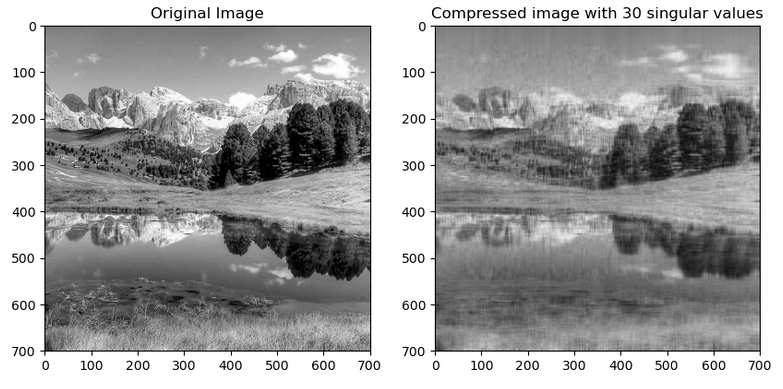
\includegraphics[width=1.0\textwidth]{svd}
    \caption{Lossy compression of a $700\times 700$ pixel grey-scale image via
      Single Value Decomposition (SVD).}
    \label{fig:svd}
  \end{figure}
  
  \begin{parts}

    \part For what values of $k$ would $A_k$ corresponds to a lossy
      compressed image? No additional explanation is necessary.

      %%% Do not change the height of this box. Your work must fit inside it.
      \makenonemptybox{0.5cm}{
        %%% Your work oes here!    
        For all $0 \le k < \operatorname{rank}(A)$
      
        %%% end of your answer    
      }
     
    \part Let $A= \sigma\mathbf{x}\mathbf{y}^T$ where
      $\mathbf{x},\mathbf{y} \in {}^n\mathbb{R}$ and $\sigma \in \R$ is nonzero. Prove that
      $\operatorname{rank}(A)=1$. \color{red}\textit{Hint:~}\color{black}
    Try constructing a $3 \times 3$ example, $A$, by choosing some
    nonzero $\sigma\in\mathbb{R}$ and
      $\mathbf{x}, \mathbf{y} \in {}^3\mathbb{R}$. This should give you the insight you 
      need to answer this question for
      general $\mathbf{x},\mathbf{y} \in {}^n\mathbb{R}$ below.

      %%% Do not change the height of this box. Your work must fit inside it.
      \makenonemptybox{9cm}{
        %%% Your work goes here!      
        Let $A = \sigma\mathbf{x}\mathbf{y}^T$ where $\mathbf{x},\mathbf{y} \in {}^3\mathbb{R}$ and $\sigma \in \R$ is nonzero. Then, WLOG, we use a $3 \times 3$ example:
        $$ A = \sigma\mathbf{x}\mathbf{y}^T = \sigma\begin{bmatrix} x_1 \\ x_2 \\ x_3 \end{bmatrix} \begin{bmatrix} y_1 & y_2 & y_3 \end{bmatrix} = \begin{bmatrix} \sigma x_1y_1 & \sigma x_1y_2 & \sigma x_1y_3 \\ \sigma x_2y_1 & \sigma x_2y_2 & \sigma x_2y_3 \\ \sigma x_3y_1 & \sigma x_3y_2 & \sigma x_3y_3 \end{bmatrix}$$
        This extends to a general $n\times n$ matrix $A$:
        $$ A = \sigma\mathbf{x}\mathbf{y}^T = \sigma\begin{bmatrix} x_1 \\ x_2 \\ \vdots \\ x_n \end{bmatrix} \begin{bmatrix} y_1 & y_2 & \cdots & y_n \end{bmatrix} = \begin{bmatrix} \sigma x_1y_1 & \sigma x_1y_2 & \cdots & \sigma x_1y_n \\ \sigma x_2y_1 & \sigma x_2y_2 & \cdots & \sigma x_2y_n \\ \vdots & \vdots & \ddots & \vdots \\ \sigma x_ny_1 & \sigma x_ny_2 & \cdots & \sigma x_ny_n \end{bmatrix}$$
        We can see that the matrix $A$ is a rank-1 matrix, since all the columns are scalar multiples of each other. Thus, $\operatorname{rank}(A) = 1$.

      
        %%% end of your answer    
      }

\newpage

\part Let
$A = \begin{bmatrix} 36 & 9 & 12 \\ -48 & -12 & -16 \\ 144 & 36 &
  48 \end{bmatrix}$. Determine the singular value decomposition
$A = \sigma {\bf x} {\bf y}^T$.

      %%% Do not change the height of this box. Your work must fit inside it.
      \makenonemptybox{3cm}{
        %%% Your work goes here!      
        $\operatorname{Col}(A) = \begin{bmatrix}
          3 & -4 & 6
        \end{bmatrix}^T$ so $\operatorname{Rank}{A} = 1$. 
        We normalize the column vector to get ${\bf x} = \begin{bmatrix} 3/\sqrt{61} \\ -4/\sqrt{61} \\ 6/\sqrt{61} \end{bmatrix}$.
        Also, we normalize $y = \begin{bmatrix} 12/13 & 3/13 & 4/13 \end{bmatrix}^T$.
        \\Thus, $A = \sigma {\bf x} {\bf y}^T = 13\sqrt{61}\begin{bmatrix} 3/\sqrt{61} \\ -4/\sqrt{61} \\ 6/\sqrt{61} \end{bmatrix} \begin{bmatrix} 12/13 & 3/13 & 4/13 \end{bmatrix}$

        %%% end of your answer    
      }

    
        
    \part\label{part:ortho} Assume  $\{\mathbf{v}_1, \mathbf{v}_2, \mathbf{v}_3\}$ is an
      orthogonal set of nonzero vectors.  Prove that the set is linearly
      independent. \label{part:orthogonal}

      %%% Do not change the height of this box. Your work must fit inside it.
      \makenonemptybox{10cm}{
        %%% Your work goes here!      
        We consider the linear combinations of the set of vectors that equals the zero vector:
        $$ \lambda_1\mathbf{v}_1 + \lambda_2\mathbf{v}_2 + \lambda_3\mathbf{v}_3 = \textbf{0}$$
        Since the set is orthogonal, we have:
        $$ 
        \begin{cases}
          \mathbf{v}_1 \cdot \mathbf{v}_2 = 0\\
          \mathbf{v}_1 \cdot \mathbf{v}_3 = 0\\
          \mathbf{v}_2 \cdot \mathbf{v}_3 = 0
        \end{cases}
        $$
        We can then take the dot product of the linear combination with $\mathbf{v}_1$, $\mathbf{v}_2$, and $\mathbf{v}_3$, also since $0\cdot\mathbf{v}_i = 0$, we have:
        $$ \mathbf{v}_1 \cdot (\lambda_1\mathbf{v}_1 + \lambda_2\mathbf{v}_2 + \lambda_3\mathbf{v}_3) = 0 \implies \lambda_1\mathbf{v}_1 \cdot \mathbf{v}_1 + \lambda_2\mathbf{v}_1 \cdot \mathbf{v}_2 + \lambda_3\mathbf{v}_1 \cdot \mathbf{v}_3 = \lambda_1\|\mathbf{v}_1\|^2 = 0$$
        Similarly, we will have:
        $$ \lambda_2\|\mathbf{v}_2\|^2 = 0 \quad \lambda_3\|\mathbf{v}_3\|^2 = 0$$
        Since $\mathbf{v}_1, \mathbf{v}_2, \mathbf{v}_3$ are non-zero vectors, we have $\|\mathbf{v}_1\|^2, \|\mathbf{v}_2\|^2, \|\mathbf{v}_3\|^2 > 0$. Thus, $\lambda_1 = \lambda_2 = \lambda_3 = 0$, which implies that the set of vectors is linearly independent.
        %%% end of your answer    
      }
      
        
    \part Consider the set $\{\mathbf{v}_1, \mathbf{v}_2, \mathbf{v}_3 \}$ from
      part~(\ref{part:ortho}).
    What property of a 4th vector $\mathbf{v}_4 \in\ ^4\R$ 
       would ensure that the extended set
      $\{\mathbf{v}_1, \mathbf{v}_2, \mathbf{v}_3, \mathbf{v}_4 \}$ spans
      ${}^4\mathbb{R}$? Give a short explanation.  Note: your explanation does not
      have to include how you would find such a $\mathbf{v}_4$.

      %%% Do not change the height of this box. Your work must fit inside it.
      \makenonemptybox{3cm}{
        %%% Your work goes here!      
        $v_4$ shall be orthogonal to all vectors in the set $\{\mathbf{v}_1, \mathbf{v}_2, \mathbf{v}_3\}$. This ensures that the extended set $\{\mathbf{v}_1, \mathbf{v}_2, \mathbf{v}_3, \mathbf{v}_4\}$ spans ${}^4\mathbb{R}$, since the set would remain linearly independent. By the Fundamental Theorem of Linear Algebra we learnt in MAT185, the size 4 set of linear independent vectors would span ${}^4\mathbb{R}$, a dim 4 vecotor space. This is beacuse the spanning set of $^4\mathbb{R}$ is at least 4, so a set of 4 linearly independent vectors would span $^4\mathbb{R}$ as it constitutes the basis thereof.
  
        %%% end of your answer    
      }



\newpage    
    
    \part Download the Jupyter notebook (see Quercus page of \textit{Assignment
      2}), which includes the python code of an SVD analysis.  Please also
    download the three example grey-scale images \textit{image1.png},
    \textit{image2.png}, and \textit{image3.png} from the same Quercus page.
    You can run the code on the
    \href{https://jupyter.utoronto.ca/hub/user-redirect/tree}{U\,of\,T Jupyter
      server}, on your own local Jupyter installation, or on the
    \href{https://undergrad.engineering.utoronto.ca/campus-facilities/engineering-computing-facility-ecf/remote-access/}{ECF
      lab PCs}. We recommend using the U\,of\,T Jupyter server, since all
    necessary packages are already installed:
    \href{https://jupyter.utoronto.ca/hub/user-redirect/tree}{https://jupyter.utoronto.ca/hub/user-redirect/tree}. For
    that, please login with your U\,of\,T credentials and click
    '\textit{upload}' to upload the IPYNB file and images. After that, you can
    open the uploaded notebook and run the Python code.
    
    Use the Jupyter Python code to analyze the provided three images. Plot the
    sorted singular values $\sigma_i$ over the index $i$ in one graph and
    discuss the results for all three provided images. Do you see a pattern of
    the result depending on each input image? 
    
    Insert your plot below.  In addition, briefly discuss which of the 3 images
    would allow for the highest and which for the lowest compression ratio by
    singular value
    decomposition. \textcolor{red}{\textit{Hint:}}\color{black}~The compression
    ratio is the uncompressed file size over the compressed file size. You don't
    need to calculate this ratio. However, think about which image would need
    the largest $k$ and which the lowest $k$ in \cref{eq:3} for an accurate
    representation of the uncompressed image, \cref{eq:2}.  For plotting
    $\sigma_i$, see the comments and plotting commands in the Jupyter
    file. Also, keep the logarithmic Y-axis for your graph.

    %%% Do not change the height of this box. Your work must fit inside it.
    \makenonemptybox{9cm}{
      %%% Add your graph and explanations here!      
      \begin{center}
  
        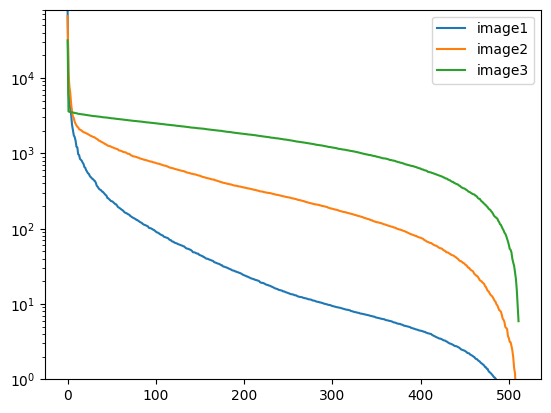
\includegraphics[width=0.6\textwidth]{graphall.png}
      \end{center}
      The graph shows the sorted singular values $\sigma_i$ over the index $i$ for the three provided images. We can see that the singular values for \textit{image1.png} decay the slowest, while the singular values for \textit{image3.png} decay the fastest. This implies that \textit{image1.png} would allow for the highest compression ratio, since it requires less $k$ for an accurate representation of the uncompressed image. On the other hand, \textit{image3.png} would allow for the lowest compression ratio, since it requires more $k$ for an accurate representation of the uncompressed image. If it has a faster decay, it means that the there would be less small singular values.
      %%% end of your answer    
    }
    
    
    \part Calculate the SVD of \textit{image1.png} with the given Jupyter code.
    For what choice of $k \in \mathbb{Z}$ would you expect a reduction in file
    size? To answer this question, estimate the memory needed to store the
    SVD-compressed image and compare it to the memory needed for the
    uncompressed 8\,bpp version of the image. \color{red}\textit{Hint:}
    \color{black} Estimate the memory size of the uncompressed image by using
    its size and given colour depth. Also note that each floating-point number
    uses 32\,Bit memory when stored.

    %%% Do not change the height of this box. Your work must fit inside it.
    \makenonemptybox{2.5cm}{
      %%% Your work goes here!      
      Size of \textit{image1.png} = $512 \times 512$ pixels, 8\,bpp.\\
      Memory needed for uncompressed image = $512 \times 512 \times 8 = 2^{21} = 2\,097\,152$ bits.\\

      \textbf{Assumption} We assume that the fullt \textit{image1.png} is rank 512. In reality it might not, but 512 is the maximum rank possible, so any $k$ as a result of this will garantee a reduction in file size.\\
          
      Memory needed for $\Sigma = k \times 32$ bits.\\
      Memory needed for each of $U, V = 2 \times k \times 512 \times 32$ bits.\\
      Total memory needed for SVD-compressed image = $k \times 32 + 2 \times  k \times 512 \times 32 = 32k + 32768k = 32800k$ bits.\\

      To expect a reduction in file size, we would need $32800k < 2\,097\,152 \implies k < 64$.


      %%% end of your answer    
    }
    
  \end{parts}
  
\end{questions}

\end{document}
